    \begin{figure}[H]
        \centering
        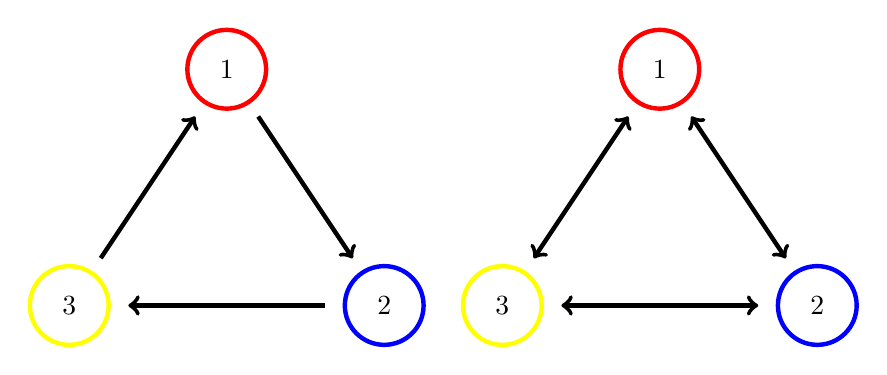
\begin{tikzpicture}
            \definecolor{cl1}{HTML}{FF0000}
            \definecolor{cl2}{HTML}{0000FF}
            \definecolor{cl3}{HTML}{FFFF00}
            \definecolor{cl4}{HTML}{FF00FF}
            \definecolor{cl5}{HTML}{00FFFF}
            \draw[ultra thick, draw=cl1] (+0,3) circle (0.5cm) node {$1$};
            \draw[ultra thick, draw=cl2] (+2,0) circle (0.5cm) node {$2$};
            \draw[ultra thick, draw=cl3] (-2,0) circle (0.5cm) node {$3$};
            \draw[ultra thick, ->] (0.4,2.40) -- (+1.6,0.60);
            \draw[ultra thick, ->] (1.25,0.0) -- (-1.25,0.0);
            \draw[ultra thick, ->] (-1.6,0.6) -- (-0.4,2.40);
            \draw[ultra thick, draw=cl1] (+5.5,3) circle (0.5cm) node {$1$};
            \draw[ultra thick, draw=cl2] (+7.5,0) circle (0.5cm) node {$2$};
            \draw[ultra thick, draw=cl3] (+3.5,0) circle (0.5cm) node {$3$};
            \draw[ultra thick, <->] (5.9 ,2.4) -- (7.1 ,0.60);
            \draw[ultra thick, <->] (6.75,0.0) -- (4.25,0.0 );
            \draw[ultra thick, <->] (3.9 ,0.6) -- (5.1 ,2.40);
        \end{tikzpicture}
        \caption{\imgtabtitle A esquerda tem-se a primeira regra adotada e à direita tem-se a segunda regra adotada para quando $\textstyle\mathcal{N}=3$.}
        \label{fig:rot3}
    \end{figure}